%=====================================================================
%	UCT EEE3017W DIGITAL ELECTRONICS NOTES 
%---------------------------------------------------------------------
%	Created by:		R.A. Verrinder
%	Date created:	December 2014
%	Date modified:	3 Jan 2015
%---------------------------------------------------------------------
%	Compile with:		arara 
%=====================================================================
%	Document properties:
%---------------------------------------------------------------------
%	Paper size:			A4
%	Margins:			1 inch margins (top,bottom,left,right)
%	Printing:			Double sided
%	Base font size:		11pt
%	Line spacing:		
%	Paragraph spacing:	10pt
%	Paragraph indent:	0pt
 %=====================================================================

\documentclass[a4paper,11pt,twoside]{book}

%---------------------------------------------------------------------
%	PACKAGES
%---------------------------------------------------------------------
\usepackage[margin = 1in]{geometry}		
\usepackage{lscape}
\usepackage{rotating}
\usepackage{hyperref}
\usepackage{hyphenat}
\usepackage{setspace}
\usepackage{hyperref}
\usepackage{titlesec}
\usepackage{lastpage}
\usepackage{fancyref}
\usepackage{fancyvrb}

\usepackage{cite}
\usepackage[usenames,dvipsnames]{xcolor}
\usepackage{graphicx}					% Can include graphics
\usepackage{float}						% Can place figures at exact places in text
\usepackage{wrapfig}					% Can wrap text around figures
\usepackage{import}

\usepackage{array}						% Can set column widths in tables
\usepackage{mdframed}					% Can draw boxes around text etc.
\usepackage{subcaption}					% Can place figures side by side
\usepackage{tikz}
\usetikzlibrary{positioning}		
\usetikzlibrary{shapes.geometric, arrows} % For block diagrams
\usetikzlibrary{circuits.logic.US} 
\usetikzlibrary{calc}
\usepackage[siunitx]{circuitikz}		% Can draw circuits
\usepackage{tikz-timing}				% Can draw timing diagrams
%\usepackage{/Users/robynverrinder/Dropbox/askmaps}					% Can draw Karnaugh maps
\usepackage{enumerate}

\usepackage{xspace}						% For box spaces
\usepackage{caption}					% Captions and subcaptions

\usepackage{fix-cm}						% Can set font size
\usepackage{color}						% Can change font color

\usepackage[scaled=0.9]{helvet}			% Helvetica font scaled
\usepackage{courier}					% Courier font
\usepackage{mathptmx}					% Times New Roman font
\usepackage{cmbright}
\normalfont 							% in case the EC fonts aren't available
\usepackage[T1]{fontenc}				% Used to switch to type 1 font encoding

\usepackage{amsmath, amsthm, amssymb}
\usepackage{datetime}					% Can use dates and times
\usepackage{gensymb}				

\usepackage{multirow}
\usepackage{hhline}

%---------------------------------------------------------------------
% 	PAGE FORMATTING
%---------------------------------------------------------------------
\parskip	= 10pt										% Paragraph spacing
\parindent 	= 0pt										% No para. indent

\captionsetup{width=0.8\textwidth,font=small,labelfont=bf}		% Caption margins 80% of text

%---------------------------------------------------------------------
%	DOCUMENT PROPERTIES
%---------------------------------------------------------------------
%\newcommand{\auth}{R.A. Verrinder}						% Author
%\newcommand{\course}{EEE3017W}							% Course code
%\newcommand{\titl}{Digital Electronics}					% Course title
%\newcommand{\stitl}{Course Textbook}					% Document title
%\newcommand{\dept}{Department of Electrical Engineering}% Department 
%\newcommand{\uni}{University of Cape Town}				% University
%\newcommand{\city}{Rondebosch, Cape Town}				% City
%\newcommand{\country}{South Africa}						% Country
%\newcommand{\aemail}{robyn.verrinder@uct.ac.za}			% Author email address

%---------------------------------------------------------------------
%	 FORMATTING FUNCTIONS
%---------------------------------------------------------------------
\mdfdefinestyle{examplebox}
{
	linecolor=black,
	linewidth=1pt,
	leftmargin=40,
	rightmargin=40,
	frametitlerule=true,
	everyline = true,
	frametitlebackgroundcolor=gray!10,
	frametitleaboveskip=3pt,
	frametitlebelowskip=9pt,
	innertopmargin=\topskip,
}

%---------------------------------------------------------------------
%	STANDARD IMAGES
%---------------------------------------------------------------------
%=====================================================================
%	Start of the document
%--------------------------------------------------------------------
\begin{document}
\graphicspath{{figs/}}
%Bold face command for programs
\newcommand{\prg}[1]{\textbf{#1}}
%Bold face & aquamarine color for locations
\newcommand{\loc}[1]{\textbf{\color{Aquamarine} #1}}
%Bold face & purple for instructions
\newcommand{\inst}[1]{\textbf{\color{Purple} #1}}
%Bold face & green for instruction location
\newcommand{\instloc}[1]{\textbf{\color{Green} #1}}
%Boldface & orange for perspective views
\newcommand{\pers}[1]{\textbf{\color{Orange} #1}}
%Ital & orange for windows in perspective
\newcommand{\wind}[1]{\emph{\color{Orange} #1}}
%Bold and brown for config
\newcommand{\conf}[1]{\textbf{\color{Brown} #1}}
%Ital and brown for config window
\newcommand{\confwind}[1]{\emph{\color{Brown} #1}}
%Bold and YellowGreen for command instruction and 20pt hspace
\newcommand{\cmd}[1]{\-\ \hspace{20pt} \textbf{\color{YellowGreen} #1}}
\chapter{Setting Up Eclipse}
\label{ch:Eclipse}

\section{Configuring Eclipse on the UCT Computers}
\label{sec:EclipseConfig}
\prg{Eclipse} is fully configured on the UCT campus computers but there are some steps that you need to remember before getting started. First plug in your STM32 board, Windows should start searching for a pre-configured driver once it's plugged in.
\includegraphics[height=3ex]{driverico}\\
\begin{figure}[htbp]
\centering
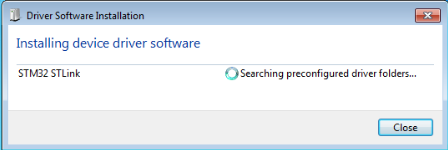
\includegraphics[width=0.6\textwidth]{driverinst}
\end{figure}
\\
Windows should eventually find the drivers and you're ready to go. Launch up Eclipse, it is important you leave the default workspace as \loc{C:\textbackslash Workspace}.
\begin{figure}[htbp]
\centering
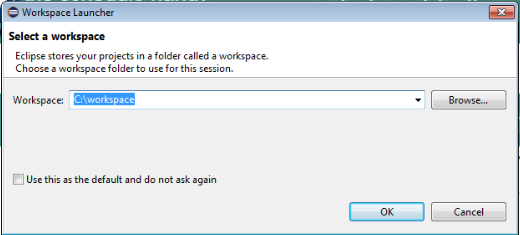
\includegraphics[width=0.8\textwidth]{workspace}
\end{figure}
\\
Then wait for \prg{Eclipse} to load up, then create a new \inst{STM32F0xx C\textbackslash C++ Project}. The compiler will load up all the relevant files and put out a pretty empty generic template. First off, build the project so you have a set of binaries (.ELF files) to work with. You Build a project by following \instloc{Project $\rightarrow$ Build All} ,or selecting \inst{Build Project} by right-clicking on the project file in the \wind{File Explorer window}.
\\
To run the code on your STM32 board, simply \inst{Debug} the project using the \conf{GDB OpenOCD Debugging} configurations. The UCT computers will auto detect the project you are working on (only if you've already built it). Conveniently, the config for \prg{OpenOCD} is auto filled out already so you can debug your code from the \pers{Debug Perspective}.
\par
{
\centering
\fbox{
\begin{minipage}{0.9\textwidth}
\justifying
\parindent=0pt
\color{Red}
If you receive an error saying \textbf{"Program file does not exist"} then you haven't pre-built your program. For the Eclipse debugger to correctly fill out the default configurations for debugging you need to have built the project first.
\par
\centering
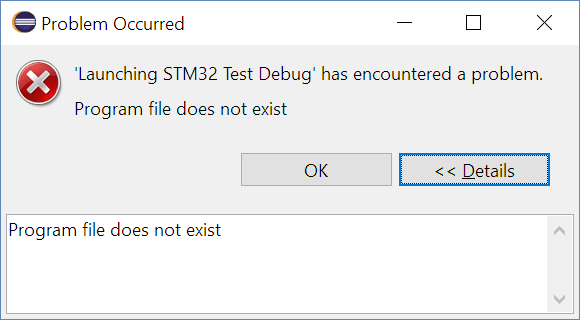
\includegraphics[width=0.5\textwidth]{programfileerror}
\\
\justifying
\parindent=0pt
\textbf{Build} your project and then in the debug configurations menu, under the \underline{\smash{C\textbackslash C++ Application}} select to \textbf{Search Project} and chose the .ELF file. You should be able to debug now
\end{minipage}
}}
\newpage
\section{TL;DR}
\label{tldr}
You might have already used your computer with your STM32 board in previous courses and you just want to get eclipse working. This is the itemized process, if you run into any problems you can use the rest of the guide as reference.
\par
\begin{enumerate}
\raggedright
\item Download Eclipse MARS for C/C++:\\
\centering \href{http://www.eclipse.org/downloads/packages/eclipse-ide-cc-developers/mars2}{\color{Blue} \underline{http://www.eclipse.org/downloads/packages/eclipse-ide-cc-developers/mars2}}
\\
\raggedright
\item In Eclipse, add the repository for GNU ARM ECLIPSE Tools:\\
\centering \instloc{Help $\rightarrow$ Install New Software $\rightarrow$ Add}
\\
\raggedright
Then in \underline{name}, fill in \textbf{GNU ARM ECLIPSE} and paste the P2P repository URL for the toolset in the \underline{location}; \url{http://gnuarmeclipse.sourceforge.net/updates} 
\\
Finally,tick and install \textbf{GNU ARM C/C++ Cross Development Tools}
\raggedright
\item From the same \textbf{Install New Software} window, add the P2P repo for the MARS CDT: \url{http://download.eclipse.org/tools/cdt/releases/8.8.1} and install:
\\
\centering \instloc{Optional Features $\rightarrow$ C/C++ GDB Hardware Debugging}
\\
\raggedright
\item Create a new C project;\\
\centering \instloc{File $\rightarrow$ New $\rightarrow$ Project $\rightarrow$ C/C++ $\rightarrow$ C Project}\\
\raggedright 
Click \textbf{Next}, choose a name for the project and make sure to select the \inst{STM32F0XX C/C++ Project} in project type and click \textbf{Next} all the way though.
\raggedright
\item Once you've made the project, build it using the \textbf{Internal Builder} which is selected by \inst{Right-Clicking} on the project;\\
\centering \instloc{Project $\rightarrow$ Properties $\rightarrow$ C/C++ Build}
\\
\raggedright
Then select \textbf{All Configurations} and choose the \textbf{Internal Builder}. Finally \inst{Right-Click} again on the project and choose \textbf{Build}.
\item Once the project has been built, configure the Debugger by \inst{Right-Clicking} on the project;\\
\centering \instloc{Debug As $\rightarrow$ Debug Configurations...}
\\
\raggedright
\inst{Double-Click} on \textbf{GBD OpenOCD Debugging} to create a new config, then in the \underline{Debugger} tab, fill in the location of your OpenOCD version (the 64-bit one), mine is: \loc{C:\textbackslash Program Files\textbackslash OpenOCD\textbackslash bin-x64\textbackslash openocd.exe}. For the OpenOCD config options use:
\\
\centering \textbf{\color{Orange} -f interface/stlink-v2.cfg -f target/stm32f0x$\_$stlink.cfg}
\\
\raggedright
And for the \underline{GDB executable} just use:
\\
\centering \textbf{\color{Orange} arm-none-eabi-gdb}
\\
\raggedright \emph{\color{Gray} If you have problems with this, see Section: \ref{sec:Debug}}
\raggedright
\item All thats left is to \inst{Apply} those settings and \inst{Debug}. Each time you alter the \textbf{main.c} file of the project you'll need to rebuild it and then debug it.
\end{enumerate}
\newpage
\section{Configuring Eclipse for the STM32}
\label{sec:eclipseconfig}
The following is a guide to configuring the \prg{Eclipse IDE} for Windows to debug the STM32F051 UCT Development board; I understand it is quite lengthy but it covers many details that are important when developing for the STM32. If your \prg{Eclipse} is already set up, skip ahead to \textbf{Section \ref{sec:Perspectives} :Perspectives in Eclipse} to see how to navigate around the Eclipse environment.
\par
After installing and configuring Eclipse there is a section explaining Eclipses' functionality and how to get the most out of your STM32 development board. This guide was written using Eclipse Mars 2 CDT 8.8.1, if you follow the steps EXACTLY it will work.
\subsection{Installation}
What you need to install and the order in which you ought to do it.
\subsubsection{gcc-arm-none-eabi}
\label{subsec:gccinst}
As with regular assembly development for the STM32F051 (hence forth the STM32), the standard arm development tools are needed to assemble our written source code (main.s) into an Assembly coded object file (main.o) and finally to link that object file to the particular memory addresses of our target processor (main.elf). 
So download and install the \textbf{\color{Brown} GCC-ARM-NONE-EABI toolset} from \href{https://vula.uct.ac.za/x/m9Z91P}{\color{Blue} \underline{\smash{Vula}}}.Otherwise get it from the  \href{https://launchpad.net/gcc-arm-embedded}{\color{Blue}\underline{\smash{official site}}}   \hspace{1pt}\footnote{\url{https://launchpad.net/gcc-arm-embedded}}.
\par
Remember that this is a 32-bit version of the development tools consisting of 32-bit executables. Even if you are running a 64-bit system you will still be using these tools. Once the files are extracted you will be prompted to \inst{"Add path to environment variable"}
\begin{figure}[hbtp]
\centering
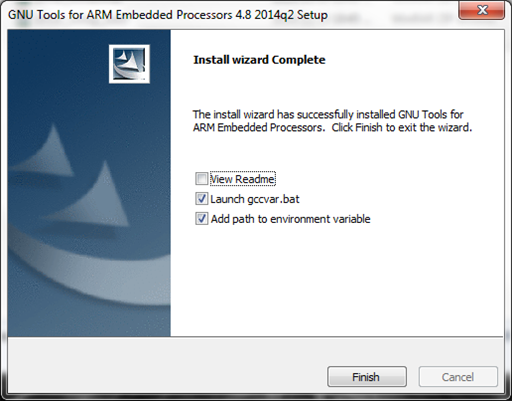
\includegraphics[width=0.6\textwidth]{gccinst}
\end{figure}
\newpage
You'll want to select this parameter, it adds the location of all the .exe's to your Windows Path Variables, in advanced system settings, so they can be run from any location without having to navigate to \loc{C:\textbackslash Program Files (x86)\textbackslash Gnu Tools Arm Embedded\textbackslash ... }
\\
You don't need to worry about the Readme or GCCVAR.bat, so deselect both and finish the installation. Included in the \textbf{\color{Brown} GNU Tools} we've just installed are debugging, compiling and linker tools provided specifically for Arm development, its' an open source tool chain which you can read about on the official \href{https://launchpad.net/gcc-arm-embedded}{\color{Blue} \underline{\smash{GCC-Arm-Embedded website}}}\hspace{1pt}\footnote{\url{https://launchpad.net/gcc-arm-embedded}}. Just to ensure that it is installed correctly (and the system path has been added to your environment variable correctly), from your command line run;
\\
\cmd{\$  arm-none-eabi-as -\hspace{2pt}- version}
\\
It should produce some details about the current GNU assembler version (this test is applicable for any of the GCC Arm tools; \textbf{ls}, \textbf{gdb} etc \ldots)
\begin{figure}[hbtp]
\centering
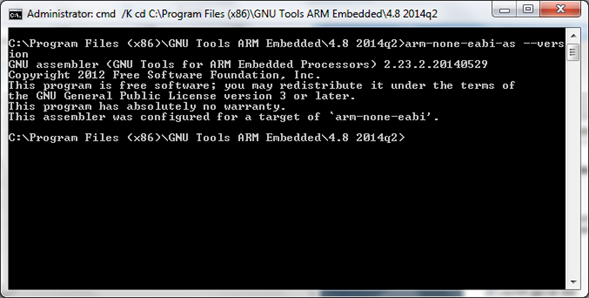
\includegraphics[width=0.6\textwidth]{gccinfo}
\end{figure}
\\
A useful trick to remember is that, within any file in windows, pressing the \inst{SHIFT key} and \inst{right clicking} inside the folder gives you the ability to open a command window (CMD) at the files current location. This isn't really important but it might come in handy.
\begin{figure}[hbtp]
\centering
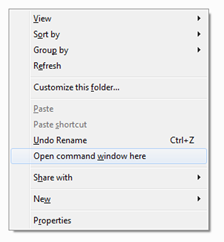
\includegraphics{cmdwindow}
\end{figure}

\newpage
\centering
\fbox{
\begin{minipage}{0.9\textwidth}
\color{Red}
\raggedright
\underline{\smash{If you receive an error}} in which the command is unrecognized it means you either have not installed the tools correctly or the environment variable path has not been appended.
\\
\centering
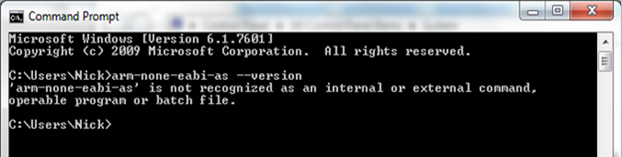
\includegraphics[width=0.9\textwidth]{armerror}
\\
\raggedright
To add the path variable you must navigate to:
\\
\cmd{Control Panel $\rightarrow$ Advanced System Settings $\rightarrow$ Environment Variables}
\\
\centering
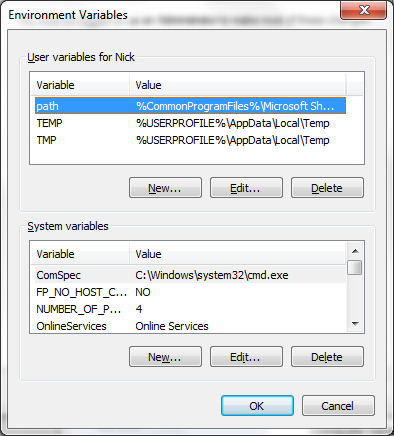
\includegraphics[width=0.6\textwidth]{envvar}
\\
\raggedright
We want to edit the \textbf{path variable} , in the variable value paste (the semi-colon is \underline{\smash{VERY IMPORTANT}}):\\
\-\ \hspace{20pt} \loc{C:\textbackslash Program Files (x86)\textbackslash GNU Tools ARM Embedded\textbackslash 4.8 2014q2\textbackslash bin;}
\\
and then accept this by pressing \inst{OK} until you are out of the system properties tab. Depending on where you installed your Tool Chain to be, this location may change so find the \textbf{bin} folder within that location and add that value to the path variable
\end{minipage}
}
\justifying
\subsubsection{Install OpenOCD}
\label{Inst:OpenOCD}
Next we need to install \textbf{\color{Brown} OpenOCD}, the \textbf{on chip debugging utility} that lets us upload our code onto our target STM32. The debugging process takes place between the ST-Link device and the target STM32. What you may not realize is that the ST-Link is actually another specially programmed STM32 microcontroller. The  ST-Link receives code from the computer, pretty much line by line, it then prepares our target STM32 to receive new code to be flashed to its memory by pulling some pins high/low in a particular order and finally it feeds our code to the target micro via a communication standard called JTAG.
\\
Download \href{https://vula.uct.ac.za/x/sRNwF6}{\color{Blue}\underline{\smash{OpenOCD-0.8.0.zip}}} from Vula or the \href{http://openocd.org/}{\color{Blue}\underline{\smash{OpenOCD Website}}}\hspace{1pt}\footnote{\url{http://openocd.org/}} and extract its' contents somewhere useful like in \loc{C:\textbackslash Program Files\textbackslash OpenOCD}
\parindent=0pt
\par
\emph{\color{Gray} Remember this location (\loc{file name}) to which you extracted OpenOCD to, mine is called OpenOCD and is in the location listed above, and yours might be different. We will need this for Debugging with Eclipse: \ref{sec:Debug}}
\par
Then navigate to \loc{C:\textbackslash Program Files\textbackslash OpenOCD\textbackslash bin-x64} and then \inst{rename executables}:
\\
\conf{openocd-x64-0.8.0.exe} to \conf{openocd.exe}
\\
\emph{\color{Gray} Windows 10 automatically includes executables in the file names so you would just change \conf{openocd-x64-0.8.0} to \conf{openocd}}
\\
This just makes things a bit easier for us. We now want to add OpenOCD's path to the Environment Variables so once again, navigate to:\\
\-\ \hspace{20pt} \instloc{Control Panel $\rightarrow$ System $\rightarrow$ Advanced System Settings $\rightarrow$ Environment Variables\ldots}
\par
Editing the path variable, we will see there is already a value for \textbf{arm-none-eabi's} tools which was added earlier in \ref{subsec:gccinst}, so after this we \underline{\smash{append}} or paste in the location of OpenOCD:
\par
\loc{C:\textbackslash Program Files\textbackslash OpenOCD\textbackslash bin-x64\textbackslash openocd.exe;}
\\
\underline{\smash{(NOTE: the semi-colon is VERY IMPORTANT)}}
\par
\centering
\fbox{
\begin{minipage}[c]{0.9\textwidth}
\color{Red}
Make sure there are \underline{\smash{no spaces}} between each subsequent path variable, only semi-colons. Mine looks like:
\\
{\raggedleft \textbf{C:\textbackslash ~MinGW\textbackslash bin;C:\textbackslash ~Program Files ~(x86)\textbackslash ~GNU Tools ~ARM Embedded\textbackslash ~Q2\textbackslash ~bin;C:\textbackslash ~Program ~Files\textbackslash ~OpenOCD\textbackslash ~bin-x64;}}
\\
If there are spaces after the semi-colons, windows won't recognize the paths as system variables and it won't work!
\end{minipage}
}
\par
\raggedright
Finally, test the path has been added correctly by running the following in the command line:\\
\cmd{\$ openocd.exe -\hspace{2pt} -version}
\\
And you should be rewarded with some more version details\ldots
\\
\begin{figure}[hbtp]
\centering
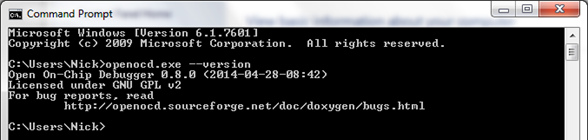
\includegraphics[width=0.7\textwidth]{openocdver}
\end{figure}
\newpage
\justifying
\subsubsection{Install ST-Link Utility}
\label{subsec:stlink}
As mentioned above, the on chip debugger makes use of the ST-Link device (we use the ST-Link V2 in particular) so we obviously need some drivers and programs for all this to work. 
Download the \href{https://vula.uct.ac.za/x/8LNN3V}{\color{Blue}\underline{\smash{ST-LINK Utility}}} from Vula or \href{http://www.st.com/content/st_com/en/products/embedded-software/development-tool-software/stsw-link004.html}{\color{Blue}\underline{\smash{ST Electronics' Site}}}\hspace{1pt}\footnote{\url{http://www.st.com/content/st_com/en/products/embedded-software/development-tool-software/stsw-link004.html}} and install the utility. This will also install the ST-Link USB drivers as well as the device utility (choose to \textbf{\color{Purple} Trust/Install} the STMicroelectronics Ports (COM \& LPT) device software)
\\
\begin{figure}[htbp]
\centering
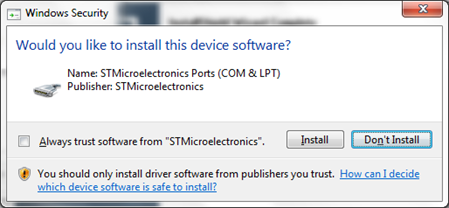
\includegraphics[width=0.6\textwidth]{installstutil}
\end{figure}
\\
For some reason the installation attempts to install the device drivers twice, just click \textbf{\color{Purple} Next} and it will take you through to the end of the installation. Now if you connect your STM32 board to your computer it should automatically detect the device (it will search for the drivers for a while and eventually give you a ready to use message)
\\
\begin{figure}[hbtp]
\centering
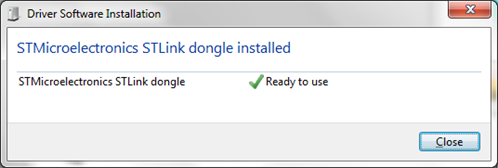
\includegraphics[width=0.6\textwidth]{stready}
\end{figure}
\parindent=0pt
\par
Whilst the USB drivers are crucial for us, the actual \conf{ST-Link utility} isn't necessary but it is very useful. If you really mess up the program running on the micro or incompletely flash a program to it, it will let you erase the memory on board your STM32 micro.
\\
Run the STM32 ST-Link Utility from wherever you installed it to and press the \inst{Connect to the Target} button 

\includegraphics[height=3ex]{conico}
. There should now be a flashing green and red LED on your board and the table in the program will be populated with memory addresses (from 0x0800000 onwards) and hexadecimal numbers.
\par
\fbox{
\begin{minipage}{0.9\textwidth}
\color{Red}
If you receive an error saying \textbf{"No ST-Link detected"} just unplug and plug back in the USB cable. When the USB driver first installs it resets the COM port which the ST-Link has previously been allocated and windows may not detect it.
\end{minipage}
}
\newpage
A console will display some info about the current state of the device as well as the devices details.  This is a powerful too which lets you manually flash programs to your micro  or erase individual memory sectors but we don't need to worry about this. All you need to know is that you can erase your chip by selecting:\\
\-\ \hspace{20pt}\instloc{Target $\rightarrow$ Erase Chip}
\\
\begin{figure}[htbp]
\centering
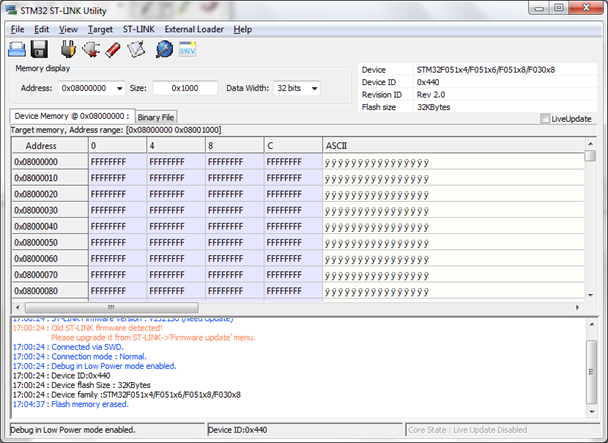
\includegraphics[width=0.8\textwidth]{stutil}
\end{figure}
\\
This cleans off any code you've flashed onto the micro and resets all memory vectors to \textbf{0xFFFFFFFFF}.
The first \underline{\smash{(and only the first)}} time you plug in your STM32 board you should update the firmware of the ST-Link, this just means we flash new (better) code onto the STM32 which operates as the ST-Link.
To do this, you will want to navigate to:\\
\-\ \hspace{20pt} \instloc{ST-Link $\rightarrow$ Firmware Update}
\\
Which opens the ST-Link Update window, first select \inst{Device Connect}. This will give you what appears to be an error about the device not being in DFU (\underline{\smash{Device Firmware Update}}) mode.\\
\begin{figure}[hbtp]
\centering
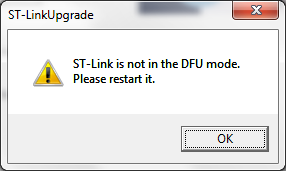
\includegraphics[width=0.4\textwidth]{dfumode}
\end{figure}
\par
This simply means the ST-Link isn't ready to have new code flashed to it, so we have to restart it. Remove the USB cable and re-plug it back in {\color{red}\underline{\smash{(don't just cycle the reset button, this won't work)}}}. The LED on the ST-Link should be a constant red now.
\newpage
Press the \inst{OK button} and then select \inst{Device Connect} again, the update utility should connect to your ST-Link now and it should display some information about what the current ST-Link firmware version is.
\begin{figure}[htbp]
\centering
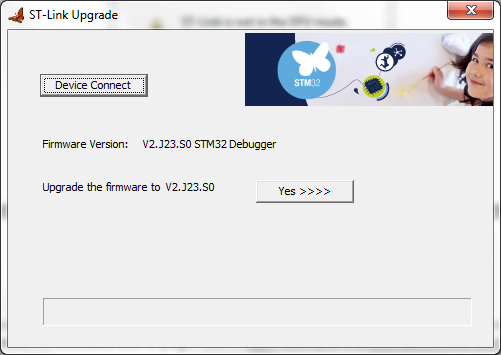
\includegraphics[width=0.7\textwidth]{firmup}
\end{figure}
\par
Then select \inst{Yes >>>>>} to update the firmware to the newest version. The Red LED on the ST-Link will flash a few times until you receive an update complete notification. 
\\
\fbox{
\begin{minipage}{0.9\textwidth}
\color{Red}
\underline{\smash{Note:}} you'll only ever need to update the firmware once when you connect the STM32 for the first time. My ST-Link has already been upgraded so my current firmware version and the version of firmware it'll update to are both V2.J23.S0 but yours will be different. Even if it's not just re-flash the software again anyway.
\end{minipage}
}
\par
\raggedright
Before continuing make sure you have disconnected 
\includegraphics[height=3ex]{disconico} the ST-Link utility from your development board.  The ST-Link works through the telnet port 3333 which can only have \underline{\smash{one program}} interfacing with it at a time, so if ST-Link utility was connected to your board then OpenOCD would not be able to connect to it. All communication ports can only be used by one program at a time, if you tried to connect OpenOCD whilst the ST-Link Utility was connect you'd receive an error that looks like:
\\
\centering
{\color{Red}
in procedure 'transport'\\
in procedure 'init'{
\parindent=0pt
\par
\justifying
\color{Gray}\emph{ A 'transport' error is almost always because you have another process already using the debugging port, we'll talk more about this later in Section \ref{sec:Debug}. So if you ever receive this sort of error, make sure all previous connections have been \textbf{\underline{\smash{terminated}}}}.
\newpage
\justifying
\color{Black}
Through the ST-Link Utility you can flash compiled programs directly to the micro controller, assuming the program has been compiled correctly. To do this, select:\\
\-\ \hspace{20pt}\instloc{Target $\rightarrow$ Program}
\\
And then navigate to a corresponding .hex or .bin file in your Eclipse Project (we will discuss this later) , its usually:\\ \loc{C:\textbackslash <Eclipse Workspace> \textbackslash <Eclipse Project Name> \textbackslash Debug \textbackslash <Eclipse Project Name>.hex}
\\
Finally press \inst{Start} to begin the flashing procedure. You'll notice that, if the program is compiled correctly, the flasher will know the entry point to the STM32s' memory (0x8000000) 
\\
\begin{figure}[htbp]
\centering
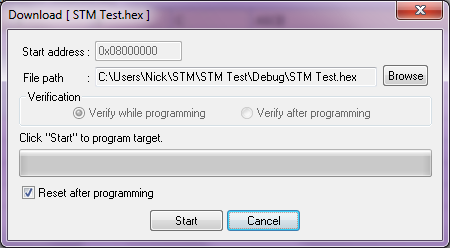
\includegraphics[width=0.6\textwidth]{stutilflash}
\end{figure}
\justifying
\par
\subsubsection{Install Java}
So, first things first, we need to set up Java. Even though we will be using C/C++ to program our micro, Eclipse is an inherent Java IDE so download the latest \href{https://www.java.com/en/download/manual.jsp}{\color{Blue}\underline{\smash{Java Runtime Edition}}}\hspace{1pt}\footnote{\url{https://www.java.com/en/download/manual.jsp}} (JRE) from the official Java website. Make sure to download the correct 64-bit or 32-bit version (depending on your operating system). 
Alternatively if you already have Java installed, you can update it through the control panel;\\
\-\ \hspace{20pt}\instloc{Control Panel $\rightarrow$ Java $\rightarrow$ Update $\rightarrow$ Update Now}
\subsubsection{Get Eclipse}
Now this is where things get a bit tricky, Eclipse is a very versatile IDE which can be configured to do almost anything but it can get pretty confusing to configure/use.
You want to download the latest\href{http://https://eclipse.org/cdt/downloads.php}{\color{Blue}\underline{\smash{Eclipse C development tool package}}}\hspace{1pt}\footnote{\url{https://eclipse.org/cdt/downloads.php}} (Eclipse CDT) at the time of writing; the latest build of Eclipse is Mars 8.8.1.\\
Eclipse is distributed as an empty package which requires a lot configuring before it does what you want it to. Extract the Eclipse CDT zip to an easily accessible folder, I recommend extracting to your \loc{C:\textbackslash file.}
\par
{\fbox{
\centering
\begin{minipage}{0.9\textwidth}
\justifying
\parindent=0pt
\color{Red}
Seeing as some of you might be doing computer programming and you use Eclipse for Java development, rename this Eclipse folder to \instloc{Eclipse-arm-dev}, to differentiate it from your Java IDE.
\end{minipage}
}}
\newpage
\parindent=0pt
Once everything is extracted, \underline{\smash{pin the Eclipse.exe to your Taskbar}} for easy access and start it up for the first time. On your first launch you will be requested to choose a workspace location where all your projects will be stored. 
\\
\justifying
It doesn't matter where you select your workspace to be but I like to keep it within my Eclipse folder, be sure to select \inst{Use this as the default and do not ask again} otherwise you will always be asked this.
\begin{figure}[htbp]
\centering
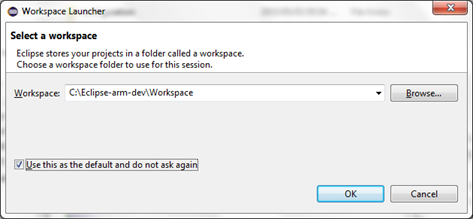
\includegraphics[width=0.6\textwidth]{eclipseworkspace}
\end{figure}
\justifying
\parindent=0pt
\par
Click \inst{OK} and wait whilst Eclipse loads up. Usually your latest project will always open up but seeing as this is our first time running the program we are greeted with a welcome message.
\par
\emph{\color{Gray} Note that when you are using the UCT lab computers you must not change the work space directory.}
\par
{
\fbox{
\color{Red}
\begin{minipage}{0.9\textwidth}
\justifying
\parindent=0pt
If Java is not correctly installed you will receive an error that Eclipse cannot open a Java DLL or a Config file, if this happens re-download and install Java, make sure that the \underline{\smash{Eclipse}} and \underline{\smash{Java}} versions you are using are both 32-bit or 64 bit. THEY MUST BE THE SAME!
\par
\centering
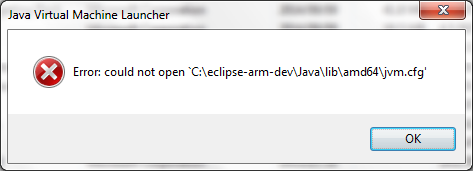
\includegraphics[width=0.6\textwidth]{JVM}
\end{minipage}
}
}
\justifying
\parindent=0pt
\par
\emph{
If Eclipse is already installed in your machine you don't need to do the above, just skip ahead to Configuring Eclipse, \ref{configeclipse}. If you are configuring a computer that already has Eclipse, make sure you are working with the C/C++ version of eclipse. To check this go to:
\\
\-\ \hspace{20pt} \instloc{Help $\rightarrow$ Install New Software $\rightarrow$ What is already installed?}
\\
In the presented list, you should see Eclipse IDE for C/C++ developers or EPP CPP Feature. These are very important as it means the Eclipse build inherently supports CDT (C Development Tools). If it lists Eclipse IDE for Java developers then the build of Eclipse is a Java version, you then need to install C/C++ Development tools if it is not listed.
\\
This guide will work for a Java environment with the CDT package installed, you can locate it at:
\url{http://www.eclipse.org/downloads/packages/eclipse-ide-cc-developers/mars2}
\\
This guide is based around a Mars build which inherently supports C/C++ development, using a Java build and adding CDT to the environment isn't recommended as I can't guarantee it will work.
}
\newpage
\subsubsection{Configuring Eclipse}
\label{configeclipse}
Seeing that we have already installed the CDT build of Eclipse the IDE will naturally support 
C/C++ compiling. We don't need to re-install the CDT package but there are some parts of it we don't already have. If you are working with eclipse and you need to add a package to the environment (not necessarily the ones we are working with now, the process is the same), you can follow these steps. You can add additional software to your eclipse build under:\\
\-\ \hspace{20pt} \instloc{Help $\rightarrow$ Install New Software}
\begin{figure}[htbp]
\centering
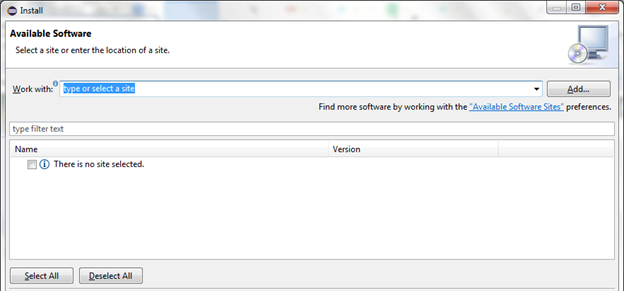
\includegraphics[width=0.7\textwidth]{installnewsoft}
\end{figure}
\\
Then \inst{Add} (adjacent to the "\underline{Work with:}" field) a new repository to work with, call it \loc{Mars CDT} and choose its location to be;\\
\textbf{\color{Orange}http://download.eclipse.org/tools/cdt/releases/8.8.1}
\par
\begin{figure}[hbtp]
\centering
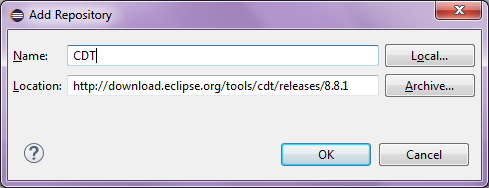
\includegraphics[width=0.7\textwidth]{addrepo}
\end{figure}
\justifying
\parindent=0pt
This is where you would \textbf{install/update} your CDT package if you needed to, expand the \inst{CDT Optional Features} and select both \underline{\smash{C/C++ GDB Hardware Debugging}} and \underline{\smash{C/C++ GCC Cross}} \underline{\smash{Compiler Support}} then click next and wait while it calculates the items which are to be installed.
\begin{figure}[htbp]
\centering
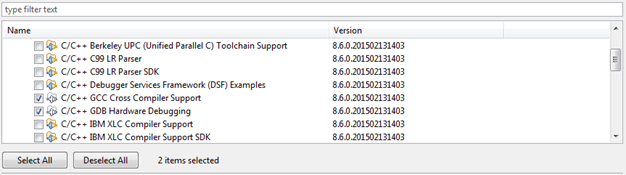
\includegraphics[width=0.8\textwidth]{GCCextra}
\end{figure}
\newpage
\parindent=0pt
\par
Click \textbf{\color{Purple} Next} and \textbf{\color{Purple} Agree} with the Eclipse Terms and Conditions (you can read them if you \underline{really} want to) and then wait while Eclipse installs the new software.
\\
\begin{figure}[hbtp]
\centering
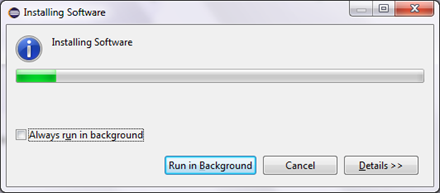
\includegraphics[width=0.7\textwidth]{inst}
\end{figure}
Eclipse will then download the \conf{GDB Hardware Debug} package which allows us to use OpenOCD from Eclipse. At the end of this installation you will be prompted to restart Eclipse. The next step is to configure Eclipse to follow the process of compiling, making, linking, assembling and then flashing our code which would otherwise be a huge, complicated task. Thankfully Eclipse is open source and Arm processors (especially the STM32 family) are very popular for embedded systems development, so people have created packages which set up eclipse for us.
\par
Once again navigate to the install new software window and add another repository, call it \inst{GNU ARM Eclipse plug-ins} and use the location: \loc{\underline{\smash{http://gnuarmeclipse.sourceforge.net/updates}}}.  Then select all the packages and install them. This will take quite a while to download/install so take this time to think about life and reflect on the decisions you've made which have led you here to Mechatronics, or think about some of the silly things you've said or done which you regret. If you feel inclined, you can read up on the \href{http://gnuarmeclipse.livius.net/blog/}{\underline{\color{Blue} \smash{Eclipse arm tools}}}\hspace{1pt}\footnote{\url{http://gnuarmeclipse.livius.net/blog/}}.  
\newpage
\fbox{
\begin{minipage}{0.9\textwidth}
\color{Red}
Recently the Eclipse Arm Tools repository has appeared to have been inaccessible so, if for whatever reason you cannot install the ARM plugin via adding the above URL to eclipse, you can download a zip file from \underline{\color{Blue} \smash{\href{http://sourceforge.net/projects/gnuarmeclipse/}{SourceForge}}}\footnote{http://sourceforge.net/projects/gnuarmeclipse/} or alternatively the same files are on \underline{\color{Blue} \smash{\href{https://vula.uct.ac.za/x/0qauui}{Vula}}}\footnote{https://vula.uct.ac.za/x/0qauui} . Extract the zip file to any easily accessible location. I extracted it to a folder on my desktop; it should contain some .JAR files.
\par
\centering
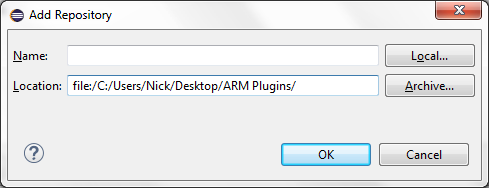
\includegraphics[width=0.6\textwidth]{localrepo}
\par
\justifying
Then in Eclipse, navigate to the \textbf{\color{Green} Install New Software} window and click on \textbf{\color{Purple} Add} a new repository, instead of filling in the URL to the update, select \textbf{\color{Purple} Local} and navigate to the location of the folder you extracted the zip to.
\par
Click \textbf{\color{Purple} Ok} and progress through the installation. Remember if you ever want to install any additional software for the Eclipse environment and you can’t find it in the official \textbf{\color{Aquamarine} Eclipse Marketplace} you may have to follow this method.
\end{minipage}
}
\par
\emph{\color{Gray} For whatever reason the SourceForge website may be down/inaccessible from your particular line, the files can be downloaded from Vula. It is far better to use the official download through their supplied URL as the plugin will automatically update through eclipse natively.}
\newpage
After installing this package and restarting Eclipse (again) you'll now see, if we choose to create a new project:\\
\-\ \hspace{20pt}\textbf{\color{Green} File $\rightarrow$ New $\rightarrow$ C Project}
\\
You’ll be presented with multiple project templates for all manner of STM32 micros. Select the \textbf{\color{Purple} STM32F0xx C/C++ Project} and choose the Cross ARM GCC toolchain (you don’t have any other options) and name your project (STM32 Test), then click next. 
\begin{figure}[htbp]
\centering
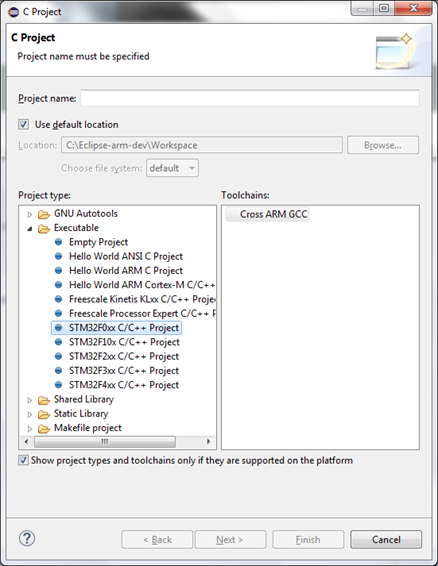
\includegraphics[width=0.6\textwidth]{cproj}
\end{figure}
\par
\fbox{
\begin{minipage}{0.9\textwidth}
\color{Red}
Obviously we choose the STM32F0xx C/C++ Project because our micro-processor falls into this category (STM32F051C) but if you were working with, say the STM32F10, you would choose a project catered for that. Those of you who've worked with the GT16 (the old micro used for this course, may she rest in peace) would recognize the name Freescale, you could even use Eclipse to debug programs written for the GT16!
\\
The Discovery boards would use the same templates (but may require additional libraries to be included) depending on what peripherals are used. In this course we use the UCT STM32 Development board, which is effectively a "Bare Metal" micro-controller breakout board so we don't have to worry about additional libraries.
\end{minipage}
}
\newpage
Following this you are presented with another window, select the Chip family to be \textbf{\color{Purple} STM32F051} (which is our micro; obviously if we were working with a different chip we would choose the appropriate one). Leave the flash, ram and clock as default. Choose content to be \textbf{\color{Purple} "Empty (add your own content)"}. The default is Blinky(Led) which we don't want because this is designed with the STM32F0 Discovery board in mind.
\\
Leave the system calls as \textbf{\color{Purple} "Freestanding (no POSIX system calls)"} which is selected by default and finally choose the Trace output to be \textbf{\color{Purple} "None (no trace output)"}.
\begin{figure}[htbp]
\centering
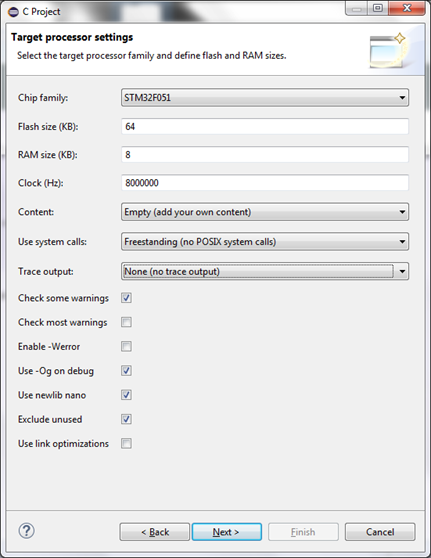
\includegraphics[width=0.7\textwidth]{targetproc}
\end{figure}
\par
Click \textbf{\color{Purple} Next}, leave the subsequent page as \textbf{\color{Purple} default}, and click \textbf{\color{Purple} Next} again. Some of these project settings may be familiar if you've compiled your C projects with a makerfile before, the Eclipse defaults are fine and I don't recommend changing them. 
At the configurations page there are some settings we will need to configure by default for all our projects, so click on \textbf{\color{Green} Advanced Settings}.
\\
\emph{\color{Gray} All the default settings are sufficient for our needs but we should discuss some of the settings involved as working on more complicated projects may produce problems that need to be addressed through more advanced feature configurations}
\newpage
This opens up a properties window with a whole bunch of settings we can change. \textbf{\color{Purple} \underline{\smash{CLICK} on}} \textbf{\color{Purple} \underline{\smash{C/C++ Build}}} (don't expand the tab, just select it) and choose to alter \textbf{\color{Purple} "[All Configurations]"} and not just \textbf{"Debug [Active]"}.
On the Builder Settings tab you can chose a Builder Type, in previous Eclipse versions an external builder was needed however this was fixed in a Luna update, ensure the \textbf{Builder Type} is set to \textbf{\color{Purple} Internal Builder}.
In \textbf{\color{Green} C/C++ Build $\rightarrow$ Settings} 
\par
In the \underline{\smash{Tool Settings tab}} there are many different subsections we can alter. Most of the default settings are sufficient for our purposes but some need to be changed.  From the top down, let's discuss them briefly because they may become important later on in the course. The \underline{\smash{Target Processor}} subsection will allow you to change what ARM family you are developing for as well as a few other parameters, leave all of these as default as they are set when configuring a new project. This is important because some processors (like the F4 and F10 families) support multi-threaded processing, but we don’t have to worry about this.
\\
\emph{\color{Gray} Just to note, if your processor supported different operating systems or instruction sets you could select an alternative other than –mthumb), by default the Endianness are configured correctly.}
\begin{figure}[hbtp]
\centering
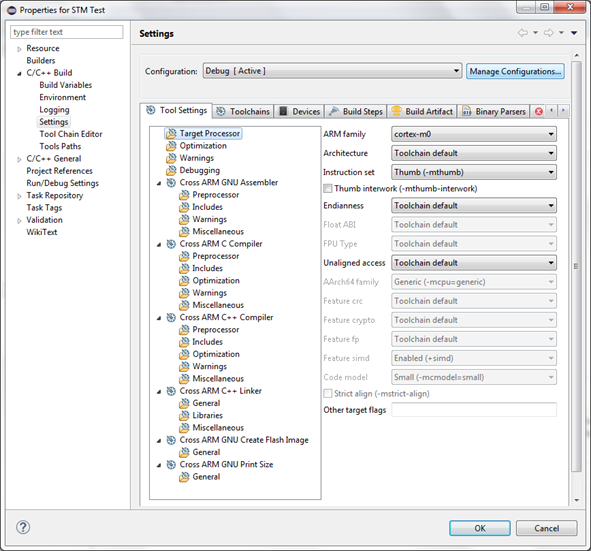
\includegraphics[width=0.8\textwidth]{toolsettings}
\end{figure}
\par
For \underline{\smash{Optimization}}, select an \textbf{\color{Purple} Optimization Level} of \textbf{\color{Purple} "None (-O0)"}. We don't want any level of code optimization just yet. Ignore Warnings and Debugging; all other tool settings can be left as their default. We don't really need to concern ourselves with their details but as you get more experienced with STM32 development in Eclipse you might want to look them up. Select \textbf{\color{Purple} OK} and \textbf{create the new project}, this project will now be used as a template for other created projects, you can alter the settings for different processors but for now the IDE is set up to only \underline{\smash{Build}} your programs from a source file written in C.
\newpage
In your Project Explorer Window (\emph{more on this in cite{sec:Navigating Eclipse}}, Eclipse provides you with a view of the Resources included in the project.  We are mainly concerned with the \textbf{\color{Aquamarine} main.c} file in which we will write our code, it's in the SRC folder.
\\
Right now the Eclipse IDE will happily recognize any STM32 Standard Peripheral Library command, but we will be working with \underline{\smash{Hardware Registry Names}}, such as \textbf{GPIOA -> IDR} for example. These are hard coded labels which represent the memory locations for the corresponding registers. At the compilation stage, Eclipse  will recognize this label to be the \textbf{memory address $0x4800 0010$}.\\
The registry labels are constructed by base memory location and the offset in the form:\\ \textbf{BASE~->~OFFSET}
\\
So here, GPIOAs' base is $0x4800 0000$ and the offset for GPIOx\_ IDR is $0x10$. You can look up these details about the STM32F0 in the reference manual.
\par
The compiler will throw \textbf{\color{Red} Symbol Unresolved errors} if you tried to include a line of code like that, so one final tool is needed, embregsysview. From:\\
\-\ \hspace{20pt} \textbf{\color{Green} Help $\rightarrow$ Eclipse Marketplace}
\\
Search for \textbf{\color{Purple} embsysregview} and install that plugin. This will allow the compiler to recognize the abstracted hardware names we will be using. We'll talk about how this plugin actually makes your life easier later in Section \cite{sec: Emgsysregview}
\begin{figure}[htbp]
\centering
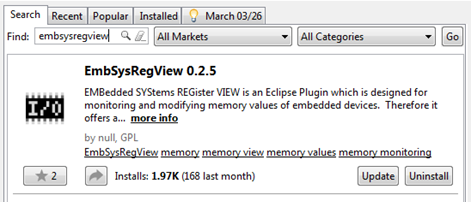
\includegraphics[width=0.6\textwidth]{embsysregview}
\end{figure}
\par
\fbox{
\begin{minipage}{0.9\textwidth}
\color{Red}
Once again, if the \textbf{\color{Purple} Eclipse Market Place} cannot link you to the Embedded Systems Registry Viewer application or it won't install correctly then download the archived files from \underline{\color{Blue} \smash{\href{https://vula.uct.ac.za/x/YXa6kS}{Vula}}} or from the \underline{\color{Blue} \smash{\href{https://sourceforge.net/projects/embsysregview/files/}{Embsysregview Source Forge Page}\footnote{https://sourceforge.net/projects/embsysregview/files/}}} and extract them into the \textbf{\color{Green} dropins} folder within your Eclipse installation file \textbf{\color{Aquamarine} C:\textbackslash Eclipse\textbackslash dropins"} or something like that.
\\
\emph{\color{Gray} This is this standard approach to installing unofficial Eclipse packages}
\\
To load up Eclipse with these additional plugins, exit and restart Eclipse completely. To check if the plugins have been detected, select: \textbf{\color{Green} $\rightarrow$ Help $\rightarrow$ Installation Details}
\\
Then choose the \textbf{\color{Purple} Plug-ins} tab and search for embsysregview. The search should produce two, unsigned plugins, another reason why it is better to install any plugins through the correct URL. This method is purely as a last resort!\\
\centering
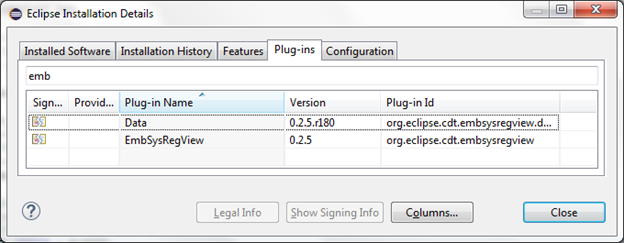
\includegraphics[width=0.7\textwidth]{regviewinst}
\end{minipage}
}
\newpage
\fbox{
\begin{minipage}{0.9\textwidth}
\color{Red}
Finally we need to tell the compiler to look at this tool and use it for recognizing some of our names we’ve given to the registers. Select: \textbf{\color{Green} $\rightarrow$ Window $\rightarrow$ Show View $\rightarrow$ Other… }
\\
Then under \textbf{\color{Purple} Debug}, double click \textbf{\color{Purple} Embsysregview} (alternatively you can just type it into the search bar). Doing this loads up the plugin into our perspective, you should have a new tab open in your perspective.
\\
\centering

\includegraphics[width=0.2\textwidth]{regviewtab}
\\
\justifying
However there isn't anything there yet because the plugin can't tell what type of µC we are looking at, so click on the settings box 
\includegraphics[height=3ex]{regviewset} which opens up the preferences page for the \textbf{Embsysreg plugin}. Fill in all the details for our STM32 as follows:
\\
\centering
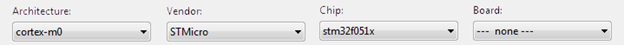
\includegraphics[width=0.9\textwidth]{regviewmicro}
\\
\justifying
Then press \textbf{\color{Aquamarine} Ok }and you should be good to go, you might have to close and reopen your already open projects (if you have any) before the compiler starts to recognize the registry names.
\\
\emph{\color{Gray} If you were using a discovery board, you'd select that in the reg view settings. This is a different installation procedure than that followed when installing the Eclipse Arm Tools plugin locally. The dropins folder allows you to implement plugins directly without any installation. This method is slightly riskier than installing the tools through the market place because we are assuming the archived .JAR files actually work. In this case they do \ldots}
\end{minipage}
}
\\
The hardware names we using are from pointer offset names defined in the particular header file used for our micro which defines the \textbf{Type\_ Defs} used, the general format is:\\
\textbf{Peripheral -> Register}\\
And mostly require a 3 stage \textbf{\color{Aquamarine} Read/Modify/Write} operation to alter its' contents. This makes life a little easier than referencing direction memory addresses.
\\
\underline{\smash{The standard operations are:}}
\begin{itemize}
\item {
\textbf{Peripheral -> Register} |= Register\_ BIT to toggle a particular bit (logical or}
\item{\textbf{Peripheral -> Register} \& = Register\_ VALUE to rewrite the registers value (logical and)} 
\item{\textbf{Peripheral -> Register} \& Register\_ BIT to check for a bit being set (bitwise and, mostly inputs)}
\end{itemize}
If you aren't sure about the naming, look up the particular Register or Bit names in \textbf{\color{Aquamarine} STM32F0xx.h\footnote{System $\rightarrow$ include $\rightarrow$ CMSIS $\rightarrow$ stm32f0xx.h}}  and familiarize yourself with the names we will be using when referring to particular peripheral registries. Alternatively you can explore the various registers you have available through the \textbf{\color{Purple} Embsysregview plugin}.
\\
Eclipse should now be happy building projects which then produces a \textbf{\color{Aquamarine} proj.elf} (in the Binaries sub folder) file which can be flashed to the STM32 via the terminal, but that's not a particularly elegant solution. Eclipse can be further configured to allow for debugging. The default settings for debugging won't work without some additional configuration.
\newpage
To compile your project, right-click on your project and select \textbf{\color{Purple} "Build Project"}; this should invoke the build process which, if no errors occur, should produce an .elf binary file with the same name as your project (see below).
\\
\emph{\color{Gray} At this stage we've made no changes to the default template created by the Eclipse Arm Plugins, it is an empty project and will do nothing if loaded onto a micro.}
\\
\fbox{
\begin{minipage}{0.9\textwidth}
\color{Red} If you get any errors at this stage make sure you have selected the External Builder and configured it to use the installed GNU Make tool.
\end{minipage}
}
\begin{figure}[htbp]
\centering
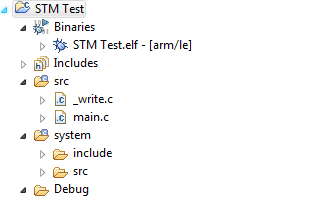
\includegraphics[width=0.3\textwidth]{projexplorer}
\end{figure}
\par
\raggedright
The \underline{\smash{Binaries}} (like the .elf and sometimes .hex or .bin files) are created during the build process, so before you build a project you've been working on, right-click on the project file and select \textbf{\color{Purple} "Clean Project"}}\color{Black}. This removes all pre-built binaries and allows for a fresh build. To build the project, select \textbf{\color{Purple} "Build Project"} directly above the Clean Project instruction.  Alternatively you can select a build configuration from the drop-down menu aside the Build Icon 
\includegraphics[height=3ex]{buildico}
\\
\fbox{
\begin{minipage}{0.9\textwidth}
\color{Red}
When building a project, in the Eclipse Console, you will see outputs from the assembler programs which you would otherwise see in the terminal. All Eclipse is doing is executing the \textbf{arm-none-eabi} tools on our behalf with a whole bunch of pre-configured parameters which are defined by which processor we are developing for.
\par
\centering
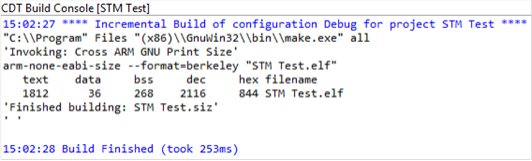
\includegraphics[width=0.6\textwidth]{buildconsole}
\\
\justifying
If you don't see this, don't worry, I'll explain how to navigate through Eclipse later.
\end{minipage}
}
\newpage
\justifying
\section{Debugging with Eclipse}
\label{sec:Debug}
The process of debugging is first to establish a connection with the debugging device. In this case it is the ST-Link V2, which connects to our computers via a full duplex USB connection. The ST-Link is made by STMicroElectronics and supports debugging on all of their micros. The benefit of using a dedicated Debug chip will be discussed later in section \cite{sec:}. Following a correction connection, the Debugger puts the target microchip (an STM32F051C in our case) into programming mode, then our debugging program starts sending the compiled code, in ASSM, to the debugger which in turn writes the code to the required registries and flash memory via J-TAG. Previously you've learnt how to debug the STM32 board using a few terminal applications, we are now going to encompass that into a single process using Eclipse.
\\
\subsection{GDB OpenOCD In Eclipse}
To configure your debug settings (or in our case create a new debug configuration), right click on your project and select:
\textbf{\color{Green} Debug As $\rightarrow$ Debug Configurations}
\par
\begin{figure}[htbp]
\centering
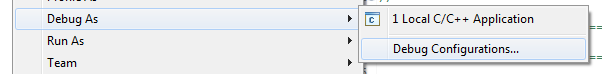
\includegraphics[width=0.8\textwidth]{debugconfig}
\end{figure}
This then brings up the \textbf{\color{Aquamarine} Debug Configurations} window, where you can select and edit your various debug configs.  Obviously we don't have any yet, so right click on \textbf{\color{Green} GDB OpenOCD Debugging} and select \textbf{\color{Purple} New}.
\\
\emph{\color{Gray} Once you've set up these configurations, every project will require you to create a new debug config but will auto-fill the settings we want.}
\begin{figure}[hbtp]
\centering
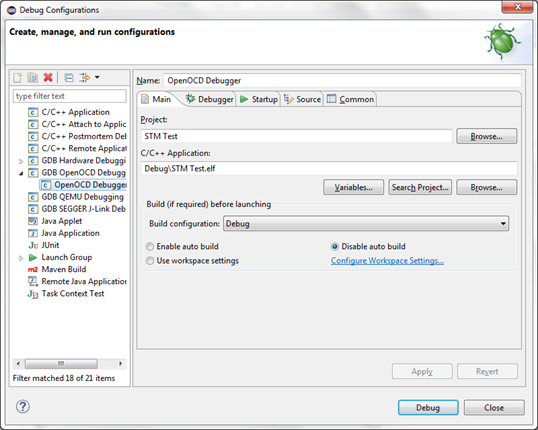
\includegraphics[width=0.7\textwidth]{debugconfigmain}
\end{figure}
\newpage
Call this new configuration \textbf{\color{Orange} "OpenOCD Debugger"} and in the \textbf{\color{Aquamarine} Main} tab you should see some parameters. By default, in the \underline{\smash{Project}} field, your project name should be filled in.
\\
\emph{\color{Gray} If you haven't yet built your project then Eclipse won't fill in anything here. You obviously want to direct the debugger to work with the \textbf{\color{Aquamarine} Project} you are currently working on. You can select \textbf{\color{Purple} Browse} to view the projects you currently have open.}
\\
For my case, it's STM Test. Similarly in the \underline{\smash{C/C++ Applications}} field it should say:
\textbf{\color{Orange} "Debug\textbackslash (Project\_ Name.elf)} or something along those lines.
\\
\emph{\color{Gray} Similarly, if you haven't built your project the program will be looking for a .elf file that doesn't exist, you can select \textbf{\color{Purple} Search Project \ldots} to select the .elf files of the built projects you've got open.}
\\
For each project you'll need to ensure you are going to be debugging the correct project, this is doubly important if you are working on multiple projects at one time. We can use the \textbf{System Variables} within Eclipse to automatically fill in the details we need, in the \underline{\smash{Project field}}, fill in:
\\
\textbf{\color{Green} \${project\_ name}}
\\
This will point to which ever project you've currently selected to debug. And finally in the \underline{\smash{C/C++ Application}} field:
\\
\textbf{\color{Green} \${project\_ loc}/Debug/\${project\_ name}.elf}
\\
Which obviously looks in the projects directory, in the Debug folder, for an .elf binary file with the same name as the project we are working on. 
\begin{figure}[hbtp]
\centering
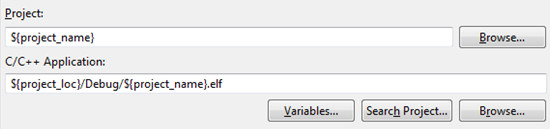
\includegraphics[width=0.8\textwidth]{debugvar}
\end{figure}
\raggedright
Next, in the \textbf{\color{Aquamarine} Debugger} tab, make sure that \textbf{\color{Orange} OpenOCD} is selected to start locally and under the \underline{\smash{Executable}} field, click the \textbf{\color{Purple} "Browse} button and locate where you have installed the \textbf{\color{Orange} OpenOCD.exe} executable.
\\
\emph{\color{Gray} OpenOCD was installed in Section: \cite{Inst:OpenOCD}}
\\
Make sure the \underline{\smash{GDB port}} is port \textbf{3333} and that the \underline{\smash{telnet port}} is \textbf{4444}. These are the communication ports on which the ST-Link listens for communications from a host device. Next, and most importantly, in the \underline{\smash{Config Options}} field, paste the following:
\\
\centering
\textbf{\color{Green} -f interface/stlink-v2.cfg –f target/stm32f0x\_ stlink.cfg}
\\
\justifying
This tells OpenOCD that we are interfacing with the St-Link, version 2, and it should use the associated configurations and secondly that the target processor is from the STM32F0x family. You can read up about why we do this on the \href{http://openocd.org/}{\underline{\smash{\color{Blue} OpenOCD website}}}\footnote{http://openocd.org/}.
\\
In the \underline{\smash{GDB Client Setup}}, make sure the Executable is:
\\
\textbf{\color{Green} arm-none-eabi-gdb}
\\
By default it could be set to just gdb, which we don't want. The Commands field should be filled out automatically but if it isn't fill it in as shown above. Then click \textbf{\color{Purple} Apply}, there are no more settings in the Debugger tab we need to change.
\newpage
\begin{figure}[htbp]
\centering
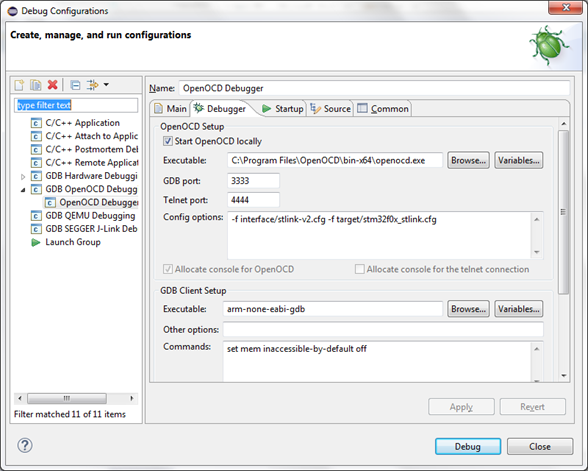
\includegraphics[width=0.7\textwidth]{debugdebugger}
\end{figure}
\par
In the \underline{\smash{Startup}} tab, scroll all the way down to the bottom and make sure a \textbf{\color{Purple} breakpoint} is set at main. I'll explain how to use/set up breakpoints later but they just tell the debugger to pause the processor at a particular point so we can see what memory values are set, we can't configure the processor to step through only 1 line of code at a time so we insert breakpoints. Finally, in the \underline{\smash{Common}} tab, select this \textbf{Debug Configuration} to Display in favorites menu and finally click \textbf{\color{Purple} Apply}.
\begin{figure}[hbtp]
\centering
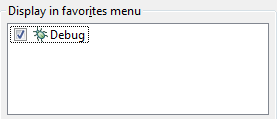
\includegraphics[width=0.4\textwidth]{debugfavorites}
\end{figure}
\par
You can now press the \textbf{\color{Purple} Debug} button; you'll be asked if you want to save some selected resources. Tick to save \textbf{"main.c"} and then select \textbf{\color{Purple} Always save resources before launching}.
\\
The first time you debug you'll be presented with a window asking to switch a \textbf{\color{Aquamarine} debug perspective}. Select yes and tick for the compiler to always remember your decision. The Debug Perspective is a different window specifically for the debugging process with a different layout.
\\ 
Your first run through will be paused (remember we put a \textbf{Breakpoint} at main, pressing the \textbf{\color{Purple}resume button} 
\includegraphics[height=3ex]{resume} which will begin execution of the code you've flashed onto the micro. We will discuss everything that can be done from this perspective later in \cite{perspectives}.
\par
You can switch between perspectives (i.e back to the \underline{\smash{C/C++ Perspective}} using the \textbf{\color{Orange} Perspectives Manager} in the top right hand corner. 
\includegraphics[height=3ex]{perspectiveico}\\
We're now going to discus what \textbf{\color{Aquamarine}perspectives} are in Eclipse and how to use them.
\newpage
\section{Perspectives in Eclipse}
\label{sec:Perspectives}
Eclipse is a multi-window IDE, meaning we can view different windows for different situations, each view is called a \textbf{\color{Aquamarine} Perspective}. By default the \textbf{\color{Aquamarine} C/C++ Perspective} is always open. 

\includegraphics[height=3ex]{CPPIco}
\\
You can customize a perspective to look like or do what ever you want, that is why Eclipse is such a powerful and useful IDE. You can open different tabs and add them to your perspective through: \textbf{\color{Green} Window $\rightarrow$ Show View $\rightarrow$ ...}
\\
The most useful part about the C/C++ Perspective is the \textbf{Project Explorer}, this is the section of the window in the far left hand side of your screen. It displays the projects you have in your working directory. You can expand the open projects and view what files are included.
\begin{figure}[htbp]
\centering
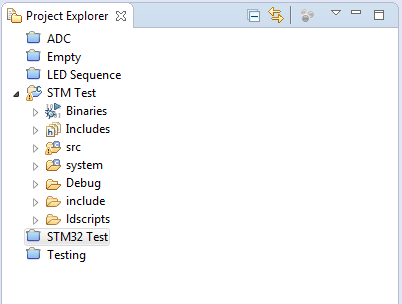
\includegraphics[width=0.4\textwidth]{projectexplorerview}
\end{figure}
\par
\fbox{
\centering
\begin{minipage}{0.9\textwidth}
\color{Red}
If you can't see the \textbf{\color{Aquamarine} Project Explorer} then display it in the perspective by selecting:\\
\-\ \hspace{20pt} \textbf{Window $\rightarrow$ Show View $\rightarrow$ Project Explorer}
\end{minipage}
}
\par
\emph{\color{Gray} It isn't really wise to have multiple projects open at any one time as this may often confuse you so be sure to close a project if you're busy working on another.}
\\
In the center of your window you'll see your \textbf{\color{Orange}Text Editor} which will most probably have the \textbf{\color{Aquamarine}main.c} source file open. If you want to look at any of your header files, you can open them up and switch between them by selecting the different tabs in the top part of this window.
\begin{figure}[hbtp]
\centering
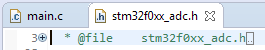
\includegraphics[width=0.4\textwidth]{files}
\end{figure}
\par
At the bottom of your screen, the \textbf{\color{Aquamarine} Console Window} is open. This window shows any returns when commands are executed, there are consoles associated with the GDB and OpenOCD programs which are displayed here. When you build your project or debug it you'll see different bits of information being displayed in the console or any errors which show up with your code at the compiling stage.
\begin{figure}[hbtp]
\centering
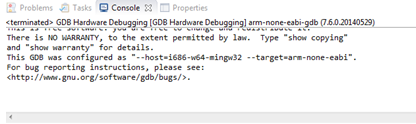
\includegraphics[width=0.6\textwidth]{console}
\end{figure}
\par
\emph{\color{Gray} All the information displayed in the console is usually to help you figure out why you're getting an error or what isn't working. It's difficult to understand initially but you'll get the hang of it.}
\newpage
To change between the different consoles you have at your disposal, use the \textbf{\color{Purple} "Display Selected Console"} drop down menu.
\includegraphics[height=3ex]{displayconsole}
\begin{figure}[htbp]
\centering
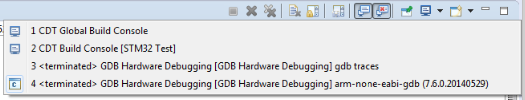
\includegraphics[width=0.7\textwidth]{displayselectedconsole}
\end{figure}
\par
If you make any changes to your perspective view, you can right click on the particular perspective in the perspective tab and \underline{\smash{save}} the changes you made.  There are lots of different ways you can set up your perspective to fit your needs so try experimenting with some. The windows are pretty self-explanatory so you can decide what you'll need or won't need and don't worry, you can always \underline{\smash{Reset}} a perspective back to its default if you don't like the changes you've made. 
In the perspectives tab you can open a new perspective to view the debugger perspective or perhaps another one. 
\includegraphics[height=3ex]{newperspectiveico}
\par
For our purposes here, you'll be using the \textbf{C/C++ Perspective} and the \textbf{Debugger Perspective}.\\\includegraphics[height=3ex]{debugperspective}\\
\emph{\color{Gray} You won't be able to see the icon for the Debug Perspective until you've run a debug process.}
\par  
The Debugger perspective is probably the most important one as this is what we use to execute the code on our STM32. It is a very powerful tool which we will now discuss. To launch the debugger from the C/C++ perspective select the debugger drop-down menu \includegraphics[height=3ex]{debugico} and choose which debug configuration you'll be using.
\begin{figure}[hbtp]
\centering
\includegraphics[width=0.4\textwidth]{debugdropdown}
\end{figure}
\\
Eclipse will automatically switch to the \textbf{Debugger perspective} once \textbf{\color{Brown} OpenOCD} has made a connection and the Debugger has access to the ST-Link. Once in the \textbf{Debug Perspective}, you are presented with a lot of windows/information. Some of it is the same as in the \textbf{C/C++ Perspective} (but they now have different functions). Starting from the top, in the \textbf{\color{Aquamarine} Debug Tab} you are shown a cascaded program tree of what is currently being executed by the program.
\begin{figure}[hbtp]
\centering
\includegraphics[width=0.8\textwidth]{debugtab}
\end{figure}
\newpage
So the tree obviously shows that you are working with the OpenOCD Debugger, you’ve executed the debug process with a particular binary (\textbf{Project\_ Name.elf}) and that we are running OpenOCD.exe and arm-none-eabi-gdb. Under Thread \# 1 is a list of "Breakpoints", breakpoints are stages of the program which, once executed, halt operation of the processor so you can inspect registry elements. By default there is only one break point (at main, seem familiar?) but we will add more later. You can set the debugger to \textbf{\color{Purple} skip all breakpoints} \includegraphics[height=3ex]{breakpointico},but that isn't all that useful.
\par
The first thing to do is \textbf{\color{Purple} Resume} execution of your program \includegraphics[height=3ex]{resumeico} and the processor will step through all the instructions you've programmed until it reaches another breakpoint when it will halt again. Once running, you can \textbf{\color{Purple} Pause} \includegraphics[height=3ex]{pauseico} your program or completely \textbf{\color{Purple} Terminate} \includegraphics[height=3ex]{terminateico} its execution. 


%---------------------------------------------------------------------
\end{document}
%---------------------------------------------------------------------